\documentclass[aspectratio=169,11pt,xcolor=dvipsnames]{beamer}
\AtBeginDocument{\special{pdf:pagesize width \the\paperwidth\space height \the\paperheight}}

% Theme
\usetheme{Madrid}
\usecolortheme{seahorse}
\setbeamertemplate{navigation symbols}{}
\setbeamertemplate{footline}{%
  \leavevmode%
  \hbox{%
    \begin{beamercolorbox}[wd=.333333\paperwidth,ht=2.5ex,dp=1.125ex,center]{author in head/foot}%
      \usebeamerfont{author in head/foot}\insertshortauthor
    \end{beamercolorbox}%
    \begin{beamercolorbox}[wd=.333333\paperwidth,ht=2.5ex,dp=1.125ex,center]{title in head/foot}%
      \usebeamerfont{title in head/foot}\insertshorttitle
    \end{beamercolorbox}%
    \begin{beamercolorbox}[wd=.333333\paperwidth,ht=2.5ex,dp=1.125ex,rightskip=1em,center]{date in head/foot}%
      \usebeamerfont{date in head/foot}\insertframenumber{} / \inserttotalframenumber
    \end{beamercolorbox}}%
  \vskip0pt%
}

% Packages
\usepackage[utf8]{inputenc}
\usepackage[T1]{fontenc}
\usepackage{lmodern}
\usepackage{graphicx}
\usepackage{booktabs}
\usepackage{tikz}
\usepackage{multicol}
\usetikzlibrary{shapes.geometric, arrows.meta, positioning, fit, backgrounds}

% Graphics path
\graphicspath{{figures/}}

% Colors
\definecolor{escpblue}{RGB}{0,51,102}
\definecolor{escpgold}{RGB}{198,146,20}
\definecolor{lightgold}{RGB}{255,243,205}
\definecolor{darkgreen}{RGB}{0,100,60}

\setbeamercolor{title}{fg=escpblue}
\setbeamercolor{frametitle}{fg=escpblue}
\setbeamercolor{structure}{fg=escpblue}
\setbeamercolor{block title}{bg=escpblue,fg=white}
\setbeamercolor{block body}{bg=escpblue!5}
\setbeamercolor{block title alerted}{bg=escpgold,fg=white}
\setbeamercolor{block body alerted}{bg=lightgold}

% Title info
\title[AI Academic Navigator]{AI Academic Navigator}
\subtitle{GPT-4 Powered Student Assessment\\in Higher Education}
\author[Jan Saro]{Jan Saro\\[0.3em]
\small Faculty of Economics and Management\\
\small Czech University of Life Sciences Prague\\[0.2em]
\scriptsize\texttt{saroj@pef.czu.cz}}
\date{}

\titlegraphic{%
\vspace{-1cm}

\begin{tikzpicture}
\node[font=\scriptsize, text=gray] {AI in Higher Education Summit $\cdot$ ESCP Business School, Paris $\cdot$ 17--18 March 2026};
\end{tikzpicture}
}

\begin{document}

% ============================================================
% TITLE SLIDE
% ============================================================
\begin{frame}[plain]
\titlepage
\end{frame}

% ============================================================
% OUTLINE
% ============================================================
\begin{frame}{Outline}
\tableofcontents
\end{frame}

% ============================================================
% MOTIVATION: SOCRATES
% ============================================================

\begin{frame}[plain]
\begin{center}
\vspace{0.5cm}

\includegraphics[width=0.75\textwidth]{Socrates.jpg}

\vspace{0.8em}
\tikz\node[draw=escpgold, fill=lightgold, rounded corners, inner sep=8pt, font=\small]{%
\begin{minipage}{0.7\textwidth}\centering
From ancient wisdom to modern AI --- the mission remains the same:\\
\textbf{help students understand themselves} to learn more effectively.
\end{minipage}};
\end{center}
\end{frame}

% ============================================================
\section{Motivation}
% ============================================================

\begin{frame}{Advantages of LLM \& GPT Models}

\begin{columns}[T]
\column{0.05\textwidth}
\column{0.90\textwidth}

{\normalsize\textbf{\color{escpblue}1. Synthesizes across multiple results}}\\[0.2em]
{\small GPT-4 can integrate data from different tests into one coherent profile.}\\[0.1em]
{\scriptsize\color{gray} Nori et al.\ (2023). \textit{Capabilities of GPT-4 on Medical Competency Examinations.} Microsoft Research.}

\vspace{0.8em}

{\normalsize\textbf{\color{escpblue}2. Explains complex results in plain language}}\\[0.2em]
{\small AI-generated medical reports were rated more understandable by patients than doctor-written ones.}\\[0.1em]
{\scriptsize\color{gray} Lyu et al.\ (2023). \textit{Translating Radiology Reports into Plain Language.} JAMA Network Open.}

\vspace{0.8em}

{\normalsize\textbf{\color{escpblue}3. Gives personalized feedback to students}}\\[0.2em]
{\small LLM explanations of assessment results matched expert tutor quality, improving self-regulated learning.}\\[0.1em]
{\scriptsize\color{gray} Kasneci et al.\ (2023). \textit{ChatGPT for Good? On LLMs in Education.} Learning \& Individual Differences.}

\column{0.05\textwidth}
\end{columns}

\vspace{1em}
\centering
\tikz\node[draw=escpgold, fill=lightgold, rounded corners, inner sep=6pt, font=\small]{%
\textbf{Our use:} All three capabilities combined in one student assessment platform.};

\end{frame}

% ============================================================

\begin{frame}[shrink=5]{Status Quo of Current Assessment Systems}

\begin{columns}[T]
\column{0.48\textwidth}
\begin{alertblock}{Current Limitations}
\begin{itemize}
    \item Delayed feedback (days/weeks)
    \item Generic, one-size-fits-all interpretation
    \item Fragmented results across tests
    \item Low engagement ($\sim$50\% completion)
    \item No cross-instrument synthesis
\end{itemize}
\end{alertblock}

\column{0.48\textwidth}
\begin{block}{Our Vision}
\begin{itemize}
    \item \textbf{Immediate} AI-generated feedback
    \item \textbf{Personalized} interpretation via GPT-4
    \item \textbf{Integrated} multi-dimensional profiles
    \item \textbf{Engaging} conversational interface
    \item \textbf{Privacy-first} client-side architecture
\end{itemize}
\end{block}
\end{columns}

\vspace{0.5em}
\centering
\tikz\node[draw=escpgold, fill=lightgold, rounded corners, inner sep=6pt, font=\small]{%
\textbf{Key Insight:} AI augments validated instruments -- it does not replace them.};

\end{frame}

% ============================================================
\section{Assessment Modules}
% ============================================================

\begin{frame}{Seven Validated Psychological Instruments}

\begin{table}
\centering
\small
\begin{tabular}{@{}lll@{}}
\toprule
\textbf{Module} & \textbf{Basis} & \textbf{Measures} \\
\midrule

Stroop Test & Stroop (1935) & Selective attention, cognitive flexibility \\
Mental Rotation & Shepard \& Metzler (1971) & Spatial visualization ability \\

VAK Assessment & Fleming (1987) & Visual / Auditory / Kinesthetic \\
Grit Scale & Duckworth (2007) & Perseverance and passion \\

Growth Mindset & Dweck (2006) & Beliefs about intelligence \\
RIASEC & Holland (1959) & Career interest typology \\

Emotional Intelligence & Goleman (1995) & Self and social awareness \\
\bottomrule
\end{tabular}
\end{table}

\vspace{0.5em}

\begin{columns}[T]
\column{0.48\textwidth}
\begin{block}{Cognitive Performance}
\begin{itemize}
    \item Stroop: 24 trials (RT + accuracy)
    \item Mental Rotation: 16 trials, 3 difficulty levels
\end{itemize}
\end{block}

\column{0.48\textwidth}
\begin{block}{Self-Report Instruments}
\begin{itemize}
    \item 5 validated questionnaires
    \item 8--12 items each
    \item Likert-scale responses
\end{itemize}
\end{block}
\end{columns}

\end{frame}

% ============================================================
\section{System Architecture}
% ============================================================

\begin{frame}[shrink=8]{Architecture: Privacy-First Design}

\begin{center}
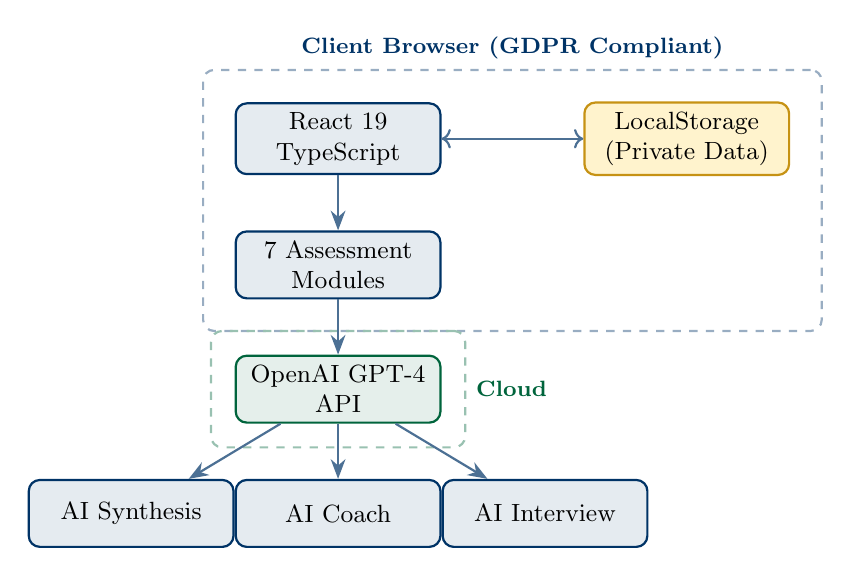
\begin{tikzpicture}[
    node distance=1cm,
    box/.style={rectangle, rounded corners, draw=escpblue, fill=escpblue!10, thick, minimum width=2.6cm, minimum height=0.85cm, align=center, font=\small},
    aibox/.style={rectangle, rounded corners, draw=darkgreen, fill=darkgreen!10, thick, minimum width=2.6cm, minimum height=0.85cm, align=center, font=\small},
    databox/.style={rectangle, rounded corners, draw=escpgold, fill=lightgold, thick, minimum width=2.6cm, minimum height=0.85cm, align=center, font=\small},
    arrow/.style={-{Stealth[length=2.5mm]}, thick, escpblue!70}
]

% Client Layer
\node[box] (react) {React 19\\TypeScript};
\node[databox, right=1.8cm of react] (local) {LocalStorage\\(Private Data)};
\node[box, below=0.7cm of react] (modules) {7 Assessment\\Modules};

% AI Layer
\node[aibox, below=0.7cm of modules] (api) {OpenAI GPT-4\\API};

% Output
\node[box, below left=0.7cm and 0cm of api] (synthesis) {AI Synthesis};
\node[box, below=0.7cm of api] (coach) {AI Coach};
\node[box, below right=0.7cm and 0cm of api] (interview) {AI Interview};

% Arrows
\draw[arrow, <->] (react) -- (local);
\draw[arrow] (react) -- (modules);
\draw[arrow] (modules) -- (api);
\draw[arrow] (api) -- (synthesis);
\draw[arrow] (api) -- (coach);
\draw[arrow] (api) -- (interview);

% Background boxes
\begin{scope}[on background layer]
    \node[draw=escpblue!40, dashed, thick, rounded corners, fit=(react)(local)(modules), inner sep=0.4cm, label={[font=\footnotesize\bfseries, text=escpblue]above:Client Browser (GDPR Compliant)}] {};
    \node[draw=darkgreen!40, dashed, thick, rounded corners, fit=(api), inner sep=0.3cm, label={[font=\footnotesize\bfseries, text=darkgreen]right:Cloud}] {};
\end{scope}

\end{tikzpicture}
\end{center}

\vspace{0.3em}
\centering\small
\textbf{Stack:} React 19 + TypeScript $\cdot$ Tailwind CSS $\cdot$ Vite $\cdot$ GPT-4 API $\cdot$ Bilingual CZ/EN

\end{frame}

% ============================================================
\section{Platform Demo}
% ============================================================

\begin{frame}{Assessment Dashboard}
\begin{columns}[T]
\column{0.55\textwidth}
\begin{center}
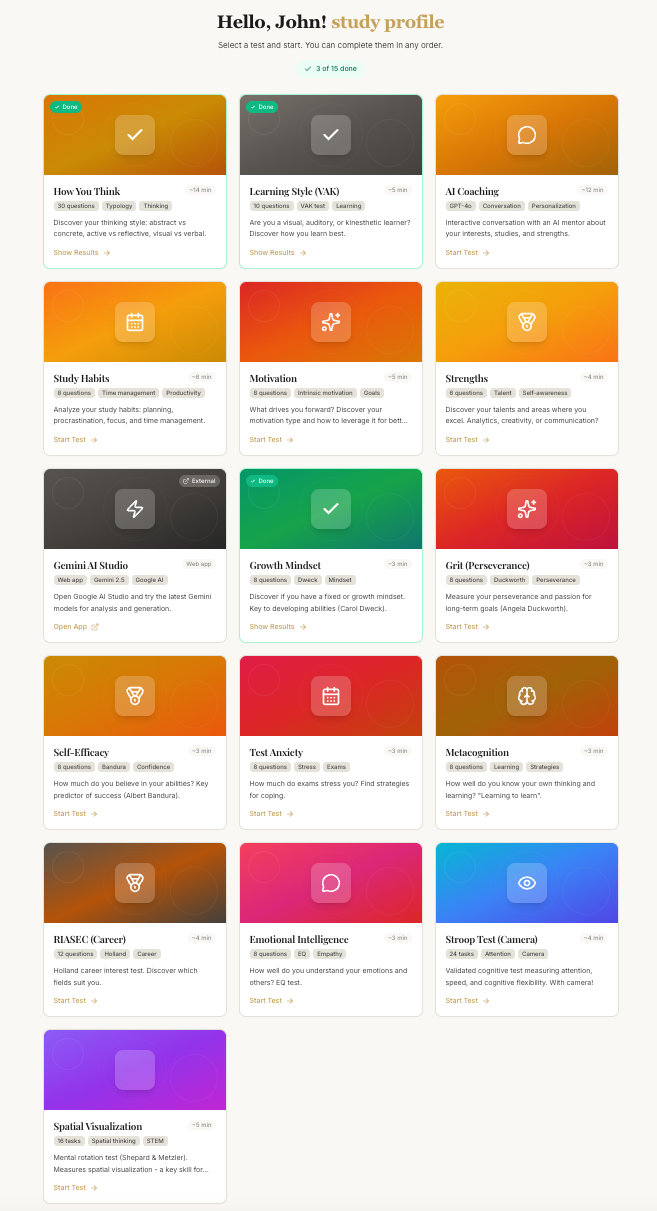
\includegraphics[width=\textwidth]{dashboard.png}
\end{center}

\column{0.42\textwidth}
\vspace{1em}
\begin{block}{Features}
\begin{itemize}
    \item Gallery-style card layout
    \item 16 cognitive \& metacognitive tests
    \item Visual progress indicators
    \item Complete in any order
    \item Estimated completion time per test
    \item Bilingual CZ/EN interface
\end{itemize}
\end{block}
\end{columns}
\end{frame}

% ============================================================

\begin{frame}{AI Conversational Interview}
\begin{columns}[T]
\column{0.45\textwidth}
\begin{center}
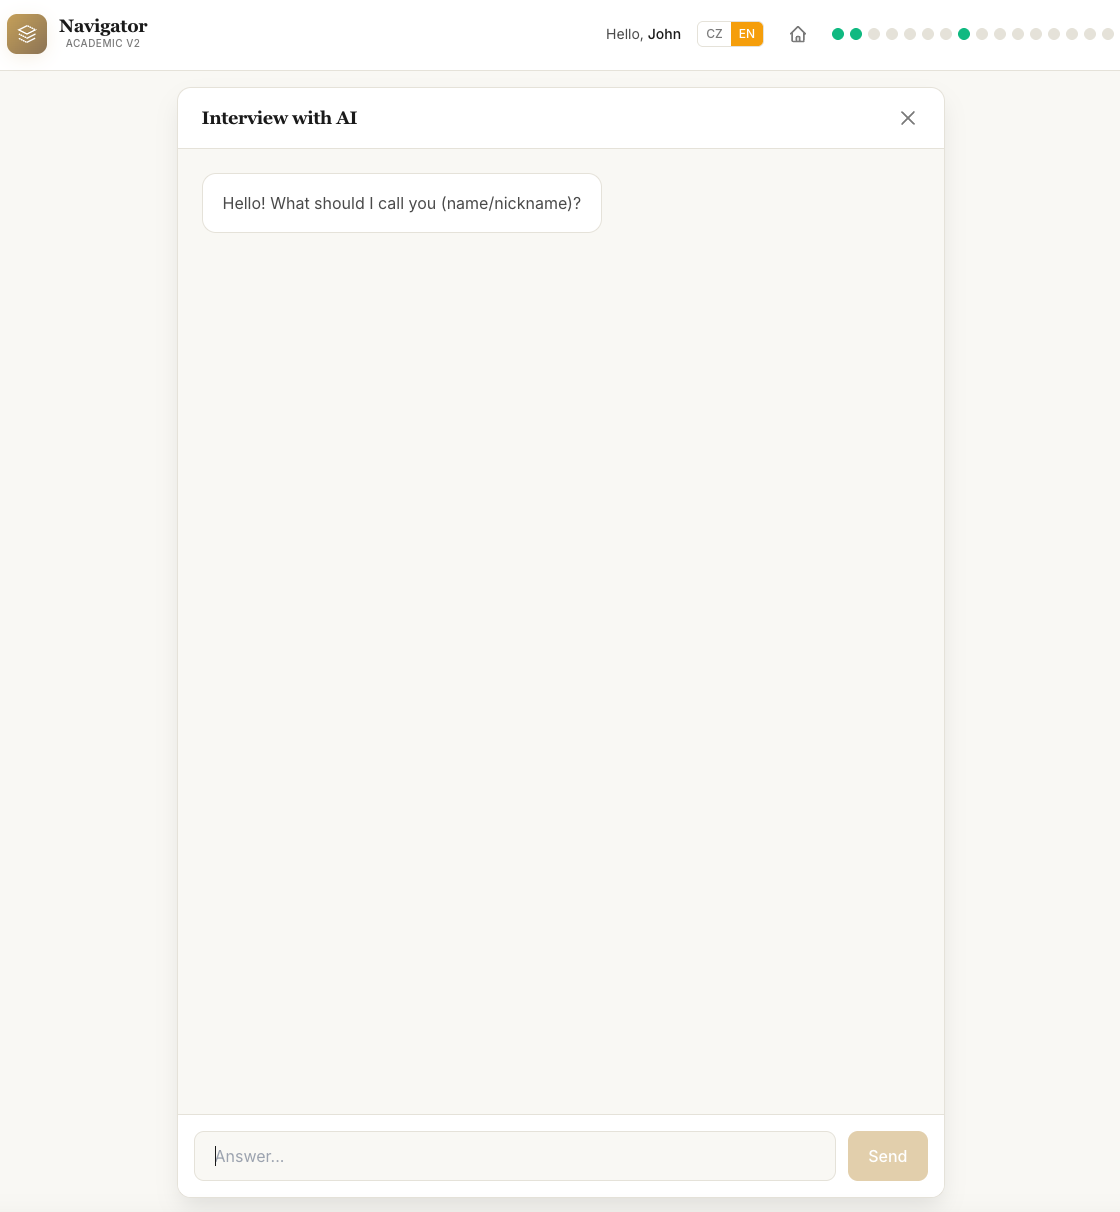
\includegraphics[width=\textwidth]{ai-interview.png}
\end{center}

\column{0.50\textwidth}
\vspace{1em}
\begin{block}{GPT-4 Powered Dialogue}
\begin{itemize}
    \item Natural conversation about interests, study habits, career goals
    \item AI adapts questions based on responses
    \item Generates comprehensive ``Student Passport''
    \item Goes beyond what structured tests capture
\end{itemize}
\end{block}

\vspace{0.5em}
\begin{alertblock}{Key Innovation}
Conversational AI explores qualitative dimensions that traditional psychometrics cannot reach.
\end{alertblock}
\end{columns}
\end{frame}

% ============================================================

\begin{frame}{AI Synthesis \& Recommendations}
\begin{center}
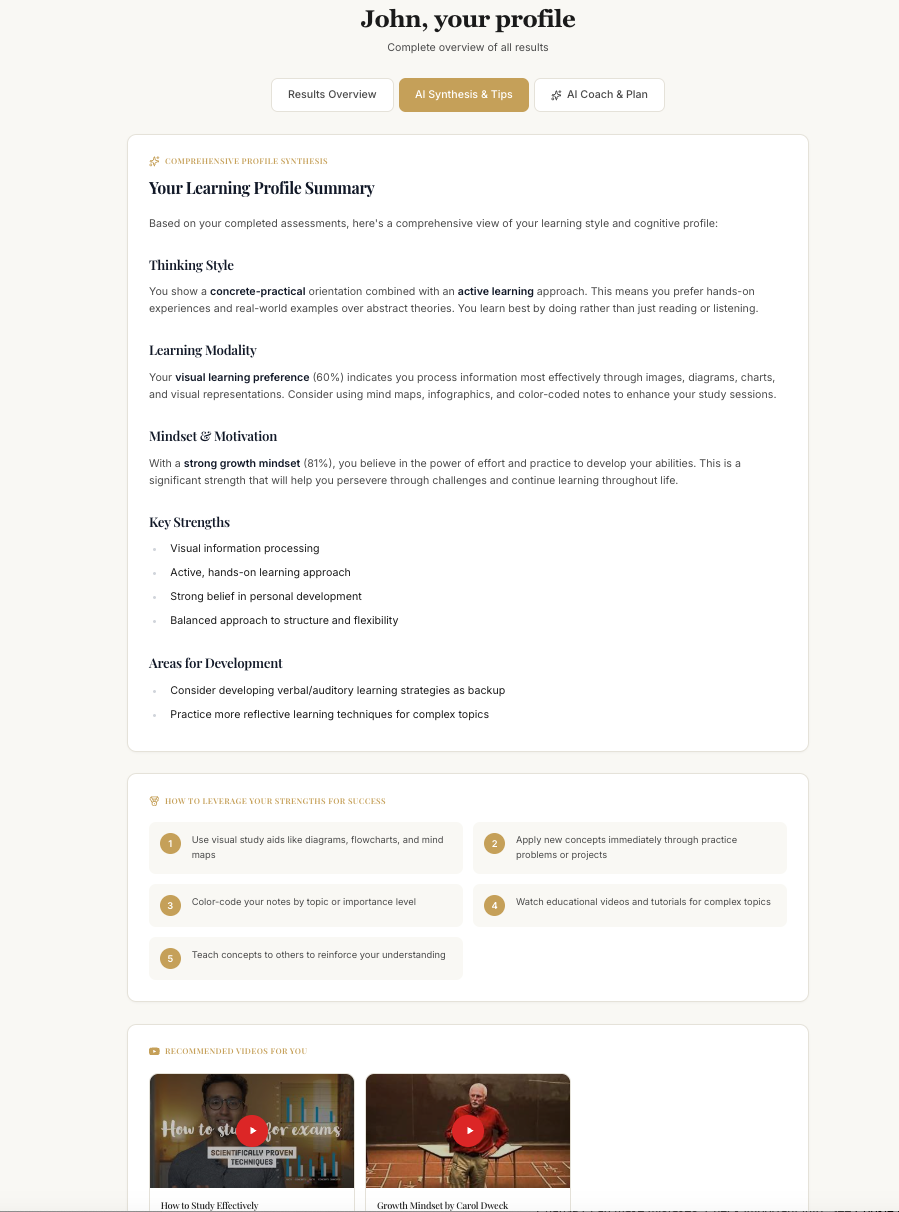
\includegraphics[width=0.72\textwidth]{ai-synthesis.png}
\end{center}

\vspace{0.2em}
\centering\small
GPT-4 integrates all results into a coherent learning profile with personalized study tips and video recommendations.
\end{frame}

% ============================================================

\begin{frame}{AI Coaching Module}
\begin{columns}[T]
\column{0.50\textwidth}
\begin{center}
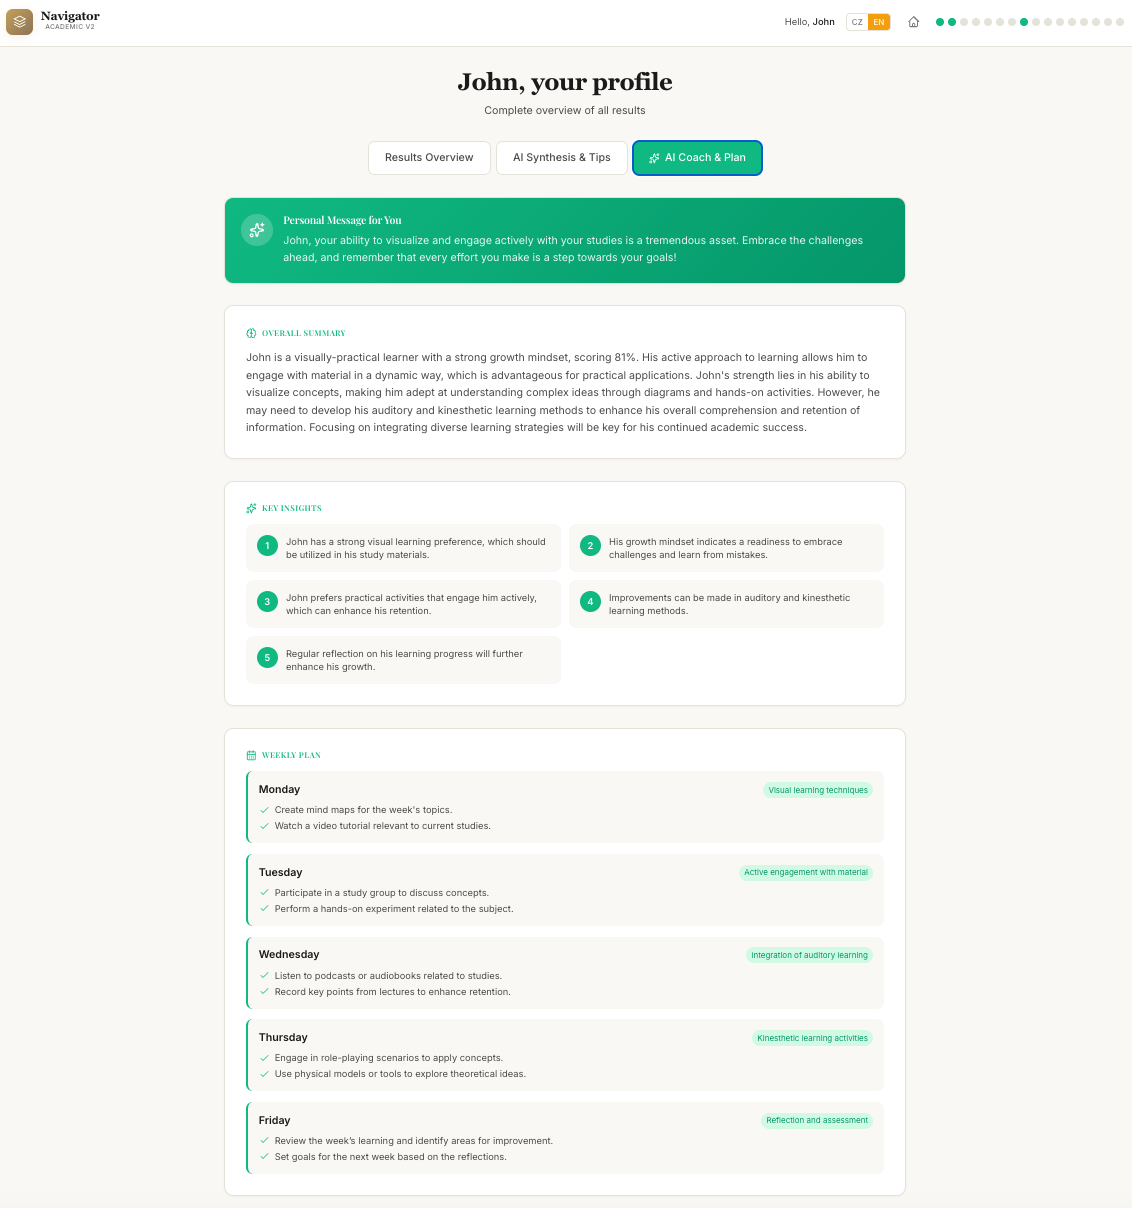
\includegraphics[width=\textwidth]{ai-coach.png}
\end{center}

\column{0.46\textwidth}
\vspace{0.5em}
\begin{block}{Personalized Action Plans}
\begin{itemize}
    \item Weekly study schedule tailored to cognitive profile
    \item Day-by-day recommendations
    \item Links activities to specific assessment results
    \item Habit tracking
    \item Motivational guidance
\end{itemize}
\end{block}

\vspace{0.3em}
\begin{exampleblock}{Example}
\small Visual learner + Growth mindset $\rightarrow$ ``Create mind maps for Monday's topics, watch video tutorials''
\end{exampleblock}
\end{columns}
\end{frame}

% ============================================================
\section{User Experience Flow}
% ============================================================

\begin{frame}{Student Journey}

\begin{center}

\begin{tikzpicture}[
    node distance=0.5cm,
    flowbox/.style={rectangle, rounded corners=4pt, draw=escpblue, fill=escpblue!15, thick, minimum width=1.9cm, minimum height=0.8cm, align=center, font=\footnotesize\bfseries},
    goldbox/.style={rectangle, rounded corners=4pt, draw=escpgold, fill=lightgold, thick, minimum width=1.9cm, minimum height=0.8cm, align=center, font=\footnotesize\bfseries},
    arrow/.style={-{Stealth[length=2.5mm]}, thick, escpblue!70}
]

\node[flowbox] (welcome) {Welcome};
\node[flowbox, right=0.7cm of welcome] (dashboard) {Dashboard};
\node[flowbox, right=0.7cm of dashboard] (assess) {Assessments};
\node[flowbox, right=0.7cm of assess] (results) {Results};
\node[goldbox, right=0.7cm of results] (synthesis) {AI Synthesis};
\node[goldbox, right=0.7cm of synthesis] (coach) {AI Coach};

\draw[arrow] (welcome) -- (dashboard);
\draw[arrow] (dashboard) -- (assess);
\draw[arrow] (assess) -- (results);
\draw[arrow] (results) -- (synthesis);
\draw[arrow] (synthesis) -- (coach);

% Loop back
\draw[arrow, dashed, escpgold] (results.south) -- ++(0,-0.6) -| (dashboard.south);

% Labels
\node[below=0.15cm of welcome, font=\tiny, text=gray] {Name entry};
\node[below=0.15cm of dashboard, font=\tiny, text=gray] {Choose tests};
\node[below=0.15cm of assess, font=\tiny, text=gray] {7 instruments};
\node[below=0.15cm of results, font=\tiny, text=gray] {Scores \& charts};
\node[below=0.15cm of synthesis, font=\tiny, text=gray] {Cross-test insights};
\node[below=0.15cm of coach, font=\tiny, text=gray] {Weekly plan};

\end{tikzpicture}
\end{center}

\vspace{0.8em}

\begin{columns}[T]
\column{0.30\textwidth}
\begin{block}{\centering Assessment}
\centering\small
7 validated instruments\\
Cognitive + Metacognitive
\end{block}

\column{0.30\textwidth}
\begin{block}{\centering AI Analysis}
\centering\small
GPT-4 cross-module synthesis\\
Pattern identification
\end{block}

\column{0.30\textwidth}
\begin{block}{\centering Action}
\centering\small
Personalized study plan\\
Habit tracking \& coaching
\end{block}
\end{columns}

\end{frame}

% ============================================================
\section{Future Directions}
% ============================================================

\begin{frame}{Future Directions}

\begin{columns}[T]
\column{0.48\textwidth}
\begin{block}{Next Steps}
\begin{itemize}
    \item \textbf{Longitudinal tracking} -- connect assessments to academic outcomes
    \item \textbf{Wearable integration} -- connect with measuring tools like smartwatches (HRV, stress)
    \item \textbf{Multi-language} -- international deployment
\end{itemize}
\end{block}

\column{0.48\textwidth}
\begin{block}{Research Agenda}
\begin{itemize}
    \item Validation of AI recommendation quality
    \item Impact on student retention
    \item Comparison with human advisor outcomes
    \item Ethical framework for AI-mediated assessment
\end{itemize}
\end{block}
\end{columns}

\vspace{1em}
\centering
\tikz\node[draw=escpblue, fill=escpblue!10, rounded corners, inner sep=8pt, font=\small]{%
\begin{minipage}{0.7\textwidth}\centering
\textbf{The future of AI in education lies not in replacement\\but in augmentation:} helping students understand themselves\\better and chart more effective learning paths.
\end{minipage}};

\end{frame}

% ============================================================
% CLOSING SLIDE
% ============================================================

\begin{frame}[plain]

\vspace{0.3cm}
\begin{center}
{\LARGE\bfseries\color{escpblue} Thank You!}\\[0.3em]
{\small Don't hesitate to connect}
\end{center}

\vspace{0.5em}

\begin{columns}[c]

\column{0.28\textwidth}
\begin{center}
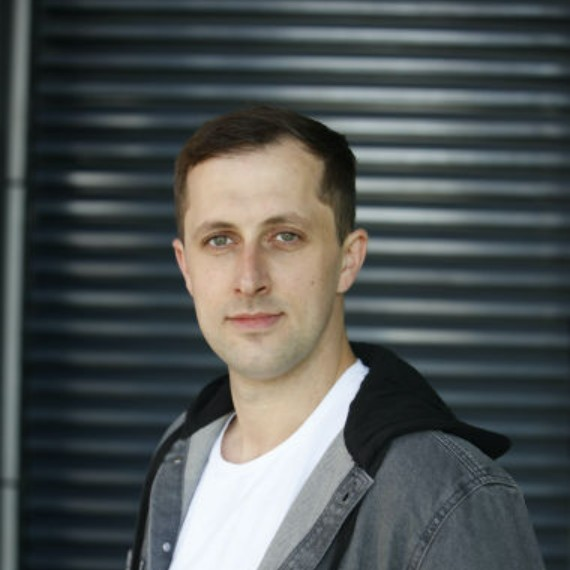
\includegraphics[width=0.75\textwidth]{jan_saro.jpeg}
\end{center}

\column{0.44\textwidth}
\begin{center}
{\large\bfseries Jan Saro}\\[0.3em]
{\small Faculty of Economics and Management}\\
{\small Czech University of Life Sciences Prague}\\[0.4em]
{\small\texttt{saroj@pef.czu.cz}}\\[0.2em]
{\small\texttt{sarojanek@gmail.com}}\\[0.6em]


\begin{tikzpicture}
\draw[escpgold, ultra thick] (-2.5,0) -- (2.5,0);
\end{tikzpicture}

\vspace{0.4em}
{\large AI Academic Navigator}\\[0.2em]
{\small GPT-4 Powered Student Assessment}
\end{center}

\column{0.24\textwidth}
\begin{center}

\includegraphics[width=0.7\textwidth]{linked_in.png}\\[0.3em]
{\scriptsize\bfseries LinkedIn}\\
{\scriptsize Connect with me!}
\end{center}

\end{columns}

\vspace{0.8em}
\begin{center}
{\footnotesize\color{gray} Session B1: AI-Powered Assessment \& Feedback $\cdot$ Chaired by Dan Levy, Harvard}\\[0.2em]
{\footnotesize\color{gray} AI in Higher Education Summit $\cdot$ ESCP Business School, Paris $\cdot$ 17--18 March 2026}
\end{center}

\end{frame}

\end{document}
